\documentclass[12pt]{article}
\setlength{\oddsidemargin}{0in}
\setlength{\evensidemargin}{0in}
\setlength{\textwidth}{6.5in}
\setlength{\parindent}{0in}
\setlength{\parskip}{\baselineskip}
\usepackage{amsmath,amsfonts,amssymb}
\usepackage{graphicx}
\usepackage{enumitem}
\usepackage[]{algorithmicx}
\usepackage{amsthm}
\usepackage{fancyhdr}
\pagestyle{fancy}
\setlength{\headsep}{36pt}
\usepackage{tkz-berge}
\usetikzlibrary{positioning, automata}

\usepackage{hyperref}

\theoremstyle{remark}
\newtheorem*{solution}{Solution}

\newcommand{\makenonemptybox}[2]{%
%\par\nobreak\vspace{\ht\strutbox}\noindent
\item[]
\fbox{% added -2\fboxrule to specified width to avoid overfull hboxes
% and removed the -2\fboxsep from height specification (image not updated)
% because in MWE 2cm is should be height of contents excluding sep and frame
\parbox[c][#1][t]{\dimexpr\linewidth-2\fboxsep-2\fboxrule}{
  \hrule width \hsize height 0pt
  #2
 }%
}%
\par\vspace{\ht\strutbox}
}
\makeatother

\begin{document}

\lhead{{\bf CSCI 3104, Algorithms \\ Problem Set 11 (60 points) - Extra Credit} }
\rhead{Name: \fbox{Michael Rogers} \\ ID: \fbox{105667404} \\ {\bf Profs.\ Hoenigman \& Agrawal\\ Fall 2019, CU-Boulder}}
\renewcommand{\headrulewidth}{0.5pt}

\phantom{Test}

\begin{small}
\textit{Advice 1}:\ For every problem in this class, you must justify your answer:\ show how you arrived at it and why it is correct. If there are assumptions you need to make along the way, state those clearly.
\vspace{-3mm} 

\textit{Advice 2}:\ Verbal reasoning is typically insufficient for full credit. Instead, write a logical argument, in the style of a mathematical proof.\\
\vspace{-3mm} 

\textbf{Instructions for submitting your solution}:
\vspace{-5mm} 

\begin{itemize}
	\item The solutions \textbf{should be typed} and we cannot accept hand-written solutions. \href{http://ece.uprm.edu/~caceros/latex/introduction.pdf}{Here's a short intro to Latex.}
	\item You should submit your work through \href{https://www.gradescope.com/courses/59294}{\textbf{Gradescope}} only.
	\item If you don't have an account on it, sign up for one using your CU email. You should have gotten an email to sign up. If your name based CU email doesn't work, try the identikey@colorado.edu version. 
	\item Gradescope will only accept \textbf{.pdf} files (except for code files that should be submitted separately on Gradescope if a problem set has them) and \textbf{try to fit your work in the box provided}. 
	\item You cannot submit a pdf which has less pages than what we provided you as Gradescope won't allow it. 
\end{itemize}
\vspace{-4mm} 
\end{small}

\hrulefill
\pagebreak
\\
\textbf{Important:} \\
There is no late due date for this extra credit assignment.
\\This assignment has 1 (Q1) coding question. 
\begin{itemize}
    \item You need to submit 1 python file.
    \item The .py file should run for you to get points and name the file as following - \\
If Q1 asks for a python code, please submit it with the following naming convention - \texttt{Lastname-Firstname-PS11-Q1.py}.
\item You need to submit the code via Canvas but the table/plot/result should be on the main .pdf.
\end{itemize}
\pagebreak

\begin{enumerate}
    
    \item (40 pts total) A good hash function $h(x)$ behaves in practice very close to the simple uniform hashing assumption analyzed in class, but is a deterministic function. That is, $h(x)=k$ each time $x$ is used as an argument to $h()$. Designing good hash functions is hard, and a bad hash function can cause a hash table to quickly exit the sparse loading regime by overloading some buckets and under loading others. Good hash functions often rely on beautiful and complicated insights from number theory, and have deep connections to pseudorandom number generators and cryptographic functions. In practice, most hash functions are moderate to poor approximations of uniform hashing.\\
	\textbf{Python code -} Consider the following two hash functions. Let $U$ be the universe of strings composed of the characters from the alphabet $\Sigma=[${\tt A}$,\dots,${\tt Z}$]$, and let the function $f(x_{i})$ return the index of a letter $x_{i}\in \Sigma$, e.g., $f(${\tt A}$)=1$ and $f(${\tt Z}$)=26$. Finally, for an $m$-character string $x\in \Sigma^{m}$, define $h_1(x) = \left(\left[\sum_{i=1}^{m}f(x_{i})\right]\!\! \mod \ell\right)$, where $\ell$ is the number of buckets in the hash table. For the other hash function,  let the function $f_2(x_{i}, a_{i})$ return $f(x_{i})*a_{i}$, where $a_{i}$ is a uniform random integer, $a_{i}\in [${\tt 0}$,\dots,${\tt $\ell$-1}$]$, and define $h_2(x) = \left(\left[\sum_{i=1}^{m}f_2(x_{i},a_{i})\right]\!\! \mod \ell\right)$. That is, the first hash function sums up the index values of the characters of a string $x$ and maps that value onto one of the $\ell$ buckets, and the second hash function is a \textbf{universal hash function}. Note that for $h_2(x)$, the $a_i$ values are chosen randomly and fixed before you start hashing. Thus $h_2(x)$ is a randomly sampled hash function from the uniform hash function family. \\
	(Your code should have the code for each of the parts below for you to receive credit for those parts.)
	
	\begin{enumerate}
	\item (16 pts) There is a txt file on Canvas that contains US Census derived last names: \\
	Using these names as input strings, first choose a uniformly random 50\% of these name strings and then hash them using $h_1(x)$ and $h_2(x)$. Produce a histogram showing the corresponding distribution of hash locations for each hash function when $\ell=5987$. Label the axes of your figure. Brief description what the figure shows about $h_1(x)$ and $h_2(x)$; justify your results in terms of the behavior of $h(x)$. 
	 
	Hint: the raw file includes information other than the name strings, which will need to be removed; and, think about how you can count hash locations without building or using a real hash table.
	
	\begin{solution}
    
    \end{solution}
    \pagebreak
	
	
	\item (4 pts) Enumerate at least 3 reasons why $h_1(x)$ is a bad hash function relative to the ideal behavior of uniform hashing.
	\begin{solution}
    1. All different permutations of a string will hash to the same location in the distribution causing many collisions. \\ \\
2. $h_1(x)$ is also a bad hash function because it uses chaining in addition to bad hashing instead of using something like open addressing. This leads to long lists of names in the same bin. \\ \\
3. There is no element of randomness and in a perfect uniform hash, randomness is how the distribution can be spread out.
    \end{solution}
	\pagebreak
	
	\item 
		(10 pts) For $h_1(x)$, produce a plot showing (i) the length of the longest chain (were we to use chaining for resolving collisions) as a function of the number $n$ of these strings that we hash into a table with $\ell=5987$ buckets. (ii) Produce another plot showing the number of collisions as a function of $\ell$. Choose prime numbers for $\ell$ and comment on how collisions decrease as $\ell$ increases. 
    \begin{solution}
    Collisions decreas as l increases because all of the values are hashing to a small part of the distribution. As the names hash after the peak, the number in each bucket decreases because at this point it is hashing only outliers.
    \end{solution}
    \pagebreak
		
	\item (10 pts) Repeat the exercise in part (c) for $h_2(x)$ and also comment on the difference in the plots produced with respect to $h_1(x)$. 
	\begin{solution}
    I had an issue with my graphs and they didn't output the correct graph because they are the same. I would say the projected difference is that $h_2(x)$ is going to have a more even distribution than $h_1(x)$ because the bins are more evenly filled than in $h_1(x)$.
    \end{solution}
    \pagebreak
	
	


	\end{enumerate}
	
	
	\item (20 pts total) Every young wizard learns the classic NP-complete problem of determining whether some unweighted, undirected graph $G=(V,E)$ contains a Hamiltonian cycle, i.e., a cycle that visits each vertex exactly once (except for the starting/ending vertex, which is visited exactly twice). The following figure illustrates a graph and a Hamiltonian cycle on it.

% ----- FIGURE :  -----
\begin{figure}[h!]
\begin{center}
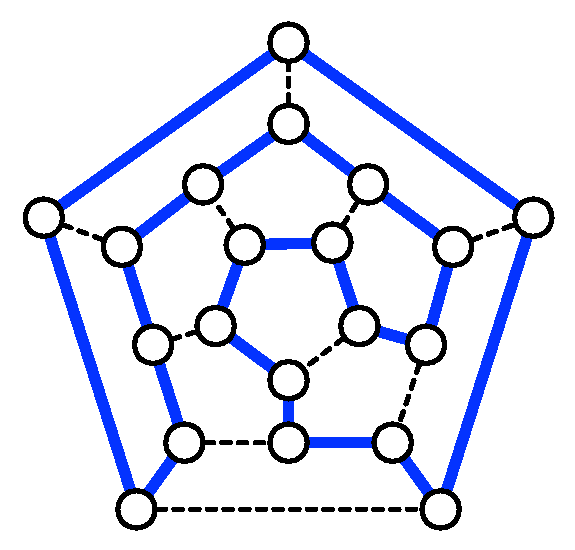
\includegraphics[scale=0.7]{hamiltonian.pdf} 
\end{center}
\vspace{-4mm}
\end{figure}
% ----------


	\begin{enumerate}
	\item (10 pts) Ginny Weasley is working on a particularly tricky instance of this problem for her Witchcraft and Algorithms class, and she believes she has written down a ``witness'' for a particular graph $G$ in the form of a path $P$ on its vertices. Explain how she should verify in polynomial time whether $P$ is or is not a Hamiltonian cycle. (And hence, demonstrate that the problem of Hamiltonian Cycle is in the complexity class NP.)
	\begin{solution}
    In order to determine if this is a hamiltonian cycle in polynomial time, we must visit every vertex along the path and count how many times each vertex has been visited. If a vertex is visited more than one time and is not the starting or ending node, then there is no way it can be apart of the hamiltonian cycle because that contradicts the definition. P must also cover every vertex in the graph. This progress would require $O(|V| + |E|)$ time and the counting can be done in $O(|V|)$ time and thus can be done in polynomial time. Since this takes polynomial time, this problem belongs to the NP class of problems.
    \end{solution}
    \pagebreak
    
	
	
	\item (10 pts) For the final exam in Ginny's class, each student must visit the Oracle's Well in the Forbidden Forest. For every bronze Knut a young wizard tosses into the Well, the Oracle will give a yes or no response as to whether a particular graph contains a Hamiltonian cycle. Ginny is given an arbitrary graph $G$, and she must find a Hamiltonian cycle on it to pass her exam.
	
	Describe an algorithm that will allow Ginny to use the Oracle to solve this problem by asking it a series of questions, each involving a modified version of the original graph $G$. Her solution must not cost more Knuts than a number that grows polynomially as a function of the number of vertices in $G$. (Hence, prove that if we can solve the Hamiltonian cycle \textit{decision} problem in polynomial time, we can solve its \textit{search} problem as well.)\\
		\begin{solution}
    Pseudocode:
\begin{verbatim}
def has_hamiltonian_cycle(G):
   if G contains no hamiltonian cycle:
      return False
   else:
      for every e in G:
         G1 = G - e
         if G1 has no hamiltonian cycle:
            e is part of cycle
         else:
            remove e from G1
      return G1
\end{verbatim}
This algorithm will go through every vertex in the graph and it will determine weather it is part of the cycle. This will determine if G has an HC $O(|E|)$ times because it is comparing every graph without each of the edges once.  $\therefore$ if the determination can be done in polynomial time, so can the search.
    \end{solution}
	
	\end{enumerate}
    
\end{enumerate}


\end{document}

